\documentclass[journal]{IEEEtran}

\hyphenation{op-tical net-works semi-conduc-tor}

\usepackage{amsmath}
\usepackage{amssymb}
\usepackage{amsthm}
\usepackage{graphicx}
\usepackage{hyperref}

\newtheorem{mydef}{Definition}
\newtheorem{mylem}{Lemma}
\newtheorem{mythm}{Theorem}
\newtheorem{myprop}{Property}
\newtheorem{mycoro}{Corollary}


\begin{document}

\title{Particle Swarm Optimization}

\author{
\IEEEauthorblockN{Daqing Yi,
Kevin D. Seppi, and Michael A. Goodrich}

\IEEEauthorblockA{Department of computer science, Brigham Young University, Provo, UT 84604 USA}
\thanks{}
}

% The paper headers
%\markboth{Journal of \LaTeX\ Class Files,~Vol.~11, No.~4, December~2012}%
%{Shell \MakeLowercase{\textit{et al.}}: Bare Demo of IEEEtran.cls for Journals}
\markboth{}{}

\maketitle

\begin{abstract}
Previous analysis of the dynamics of particle swarm optimization has often relied on either the assumption of ``stagnation'' (a state where the swarm ceases make progress), the removal of random effects, or both.
In this paper we use a newer tool for the analysis of system dynamics, specifically the concept of Input to State Stability (ISS).
ISS allows us to make statements about the behavior of the swarm not clearly address in previous analysis, specifically bounds on particle and swam behavior.
We can also do so before stagnation and with random affect fully accounted for. 
\end{abstract}

\begin{IEEEkeywords}
Particle swarm optimization
\end{IEEEkeywords}

\IEEEpeerreviewmaketitle

\section{Introduction}

\begin{frame}{Modeling human intent}{Path Planning}
THe problem in modeling human intent
\begin{itemize}
\item incomparability in objectives
\item conflict in objectives
\item hardness in weighing the objectives
\item vagueness in importance selection
\end{itemize}
\begin{figure}
\centering
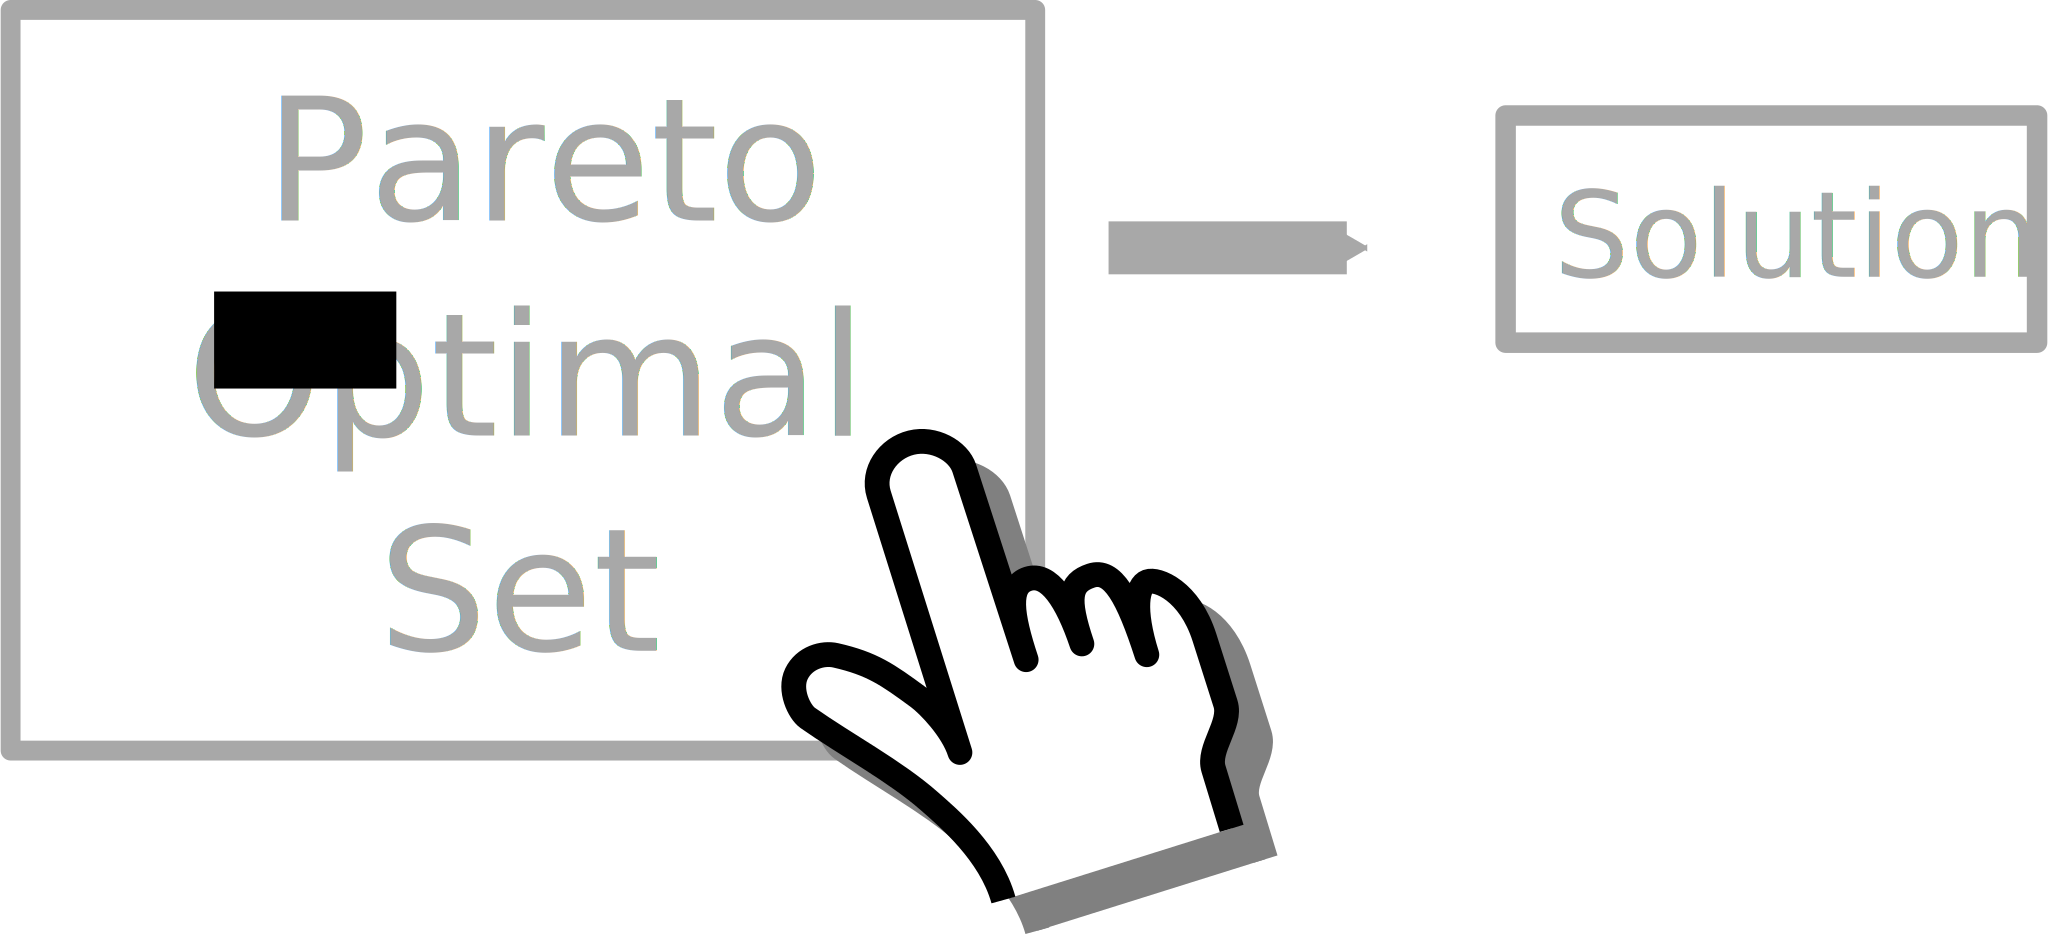
\includegraphics[width=0.6\linewidth]{figure/human_interactive_moo}
%\caption{}
\label{fig:human_interactive_moo}
\end{figure}
\end{frame}

\begin{frame}{Pareto Optimal}{}
\end{frame}

\section{Related work}

\begin{frame}{Graph based approach}{Related work}
Multi-objective A$ ^{*}$
\end{frame}

\begin{frame}{Point-equivalence based approach}{Related work}
\end{frame}



\section{Particle analysis}
\label{sec:particle}

In this section, we analyze the behavior of a single particle in a swarm.
In a single stagnation, the global best is unchanged.
Thus we make the global best as the constant.
We are interested with 
\begin{itemize}
\item whether the particle converges to the global best;
\item and the probability that the particle find a new global best.
\end{itemize}

In order to understand how the particle converges to the global best, we let $ x^{G} $ be the reference position and get Equation \eqref{eq:rel_gb}.

\begin{equation}
\label{eq:rel_gb}
\begin{aligned}
\begin{bmatrix}
v(k+1) \\
x(k+1) - x^{G}
\end{bmatrix}
 = A(k) 
\begin{bmatrix}
v(k) \\
x(k) - x^{G}
\end{bmatrix}
+ B(k) 
\begin{bmatrix}
0 \\
x^{P}(k) - x^{G}
\end{bmatrix}
\end{aligned}
\end{equation}

By Theorem \ref{coro:state_bound}, we know that $ \lVert x(k) - x^{G} \rVert $ indicates the distance to the global best, which depends on  $ \lVert x^{P}(k) - x^{G} \rVert $.

\subsection{Unimodal fitness distribution}

A unimodal fitness distribution is most typical.
It provides a partial monotonic form and most of the cases the final convergence happens on a unimodal fitness distribution.
Any other form can usually be viewed as a combination of unimodalities as well.

When the global best is already the optimal solution, there is no chance for the particle to find a better solution and trigger a new global best.
The particle should gradually converge to the global best if the position update component is input-to-state stable, as in Lemma \ref{lem:singleHill:particle:converge}.

\begin{mylem}
\label{lem:singleHill:particle:converge}
In a unimodal case, when $ x^{G} = x^{*} $, the particle will converge to $ x^{G} $ if the update component of the particle is input-to-state stable.
\begin{proof}
When $ x^{G} = x^{*} $, the input update component is also input-to-state stable.
The serial connection of two ISS components still reserves input-to-state stability.
As the input is zero by $ \lVert x^{G} - x^{*} \rVert = 0 $, $ x(k) - x^{*} $ will converge to zero.
\end{proof}
\end{mylem}

When the global best is not yet the optimal solution, the convergence of the particle cannot be guaranteed.
If the particle accidentally reaches into a region that the fitness is better than the current global best, a new global best is found.
The particle might either runs stochastically in a region that the fitness is worse than both the personal best and the global best.
If the particle at least gets into a position that is better than the current personal best, the personal best will be updated. 
We notice that the particle should never stop at the current global best $ x^{G} $, which is stated in Lemma \ref{lem:singleHill:particle:nonstop}.

\begin{mylem}
\label{lem:singleHill:particle:nonstop}
In a unimodal case, if $ x^{G} \not = x^{*} $, a particle will never stop at $ x^{G} $. 
\footnote{The precision cut-off in implementation is ignored.}
\begin{proof}
Consider the velocity $ v(k+1) $ consists of two parts, inertia $ \chi v(k) $ and attractive force $ \chi \phi^{P} (x^{P}(k) - x(k) ) + \chi \phi^{G} ( x^{G} - x(k) ) $.
While the particle moves into $ x^{G} $, the attractive force becomes zero but the inertia still exists, due to the velocity moves the particle into this current position.
\end{proof} 
\end{mylem}

By Lemma \ref{lem:singleHill:particle:nonstop}, we can prove that the particle will finally get to a position that is at least better than the current global best if given enough run time.
We have Theorem \ref{thm:singleHill:particle:better}.

\begin{mythm}
\label{thm:singleHill:particle:better}
In a unimodal case, the particle will almost surly find a $ \hat{x^{*}} $ that $ f(\hat{x^{*}}) > f(x^{G}) $ if $ f( x^{G} ) < f( x^{*}) $.
\begin{proof}
Because the particle cannot stop at $ x(k) = x^{G} = x^{P} $.
It will finally arrives into a region that $ f(x) > f(x^{G}) $.

As in Figure \ref{fig:categorize_regions}, the solution space will be divided into three types of regions by the global best and the personal best.
\begin{itemize}
\item $ f(x) > f(x^G) $
Once a particle gets into this region, it updates both global best and personal best. 
It becomes a leader of the swarm.
\item $ f(x^{G}) > f(x) > f(x^{P}) $
Once a particle gets into this region, it updates only the personal best.
The solution space is then re-divided.
\item $ f(x) < f(x^{P}) $
When a particle is in this region, it only moves as a random walk.
\end{itemize}

\begin{figure}
\centering
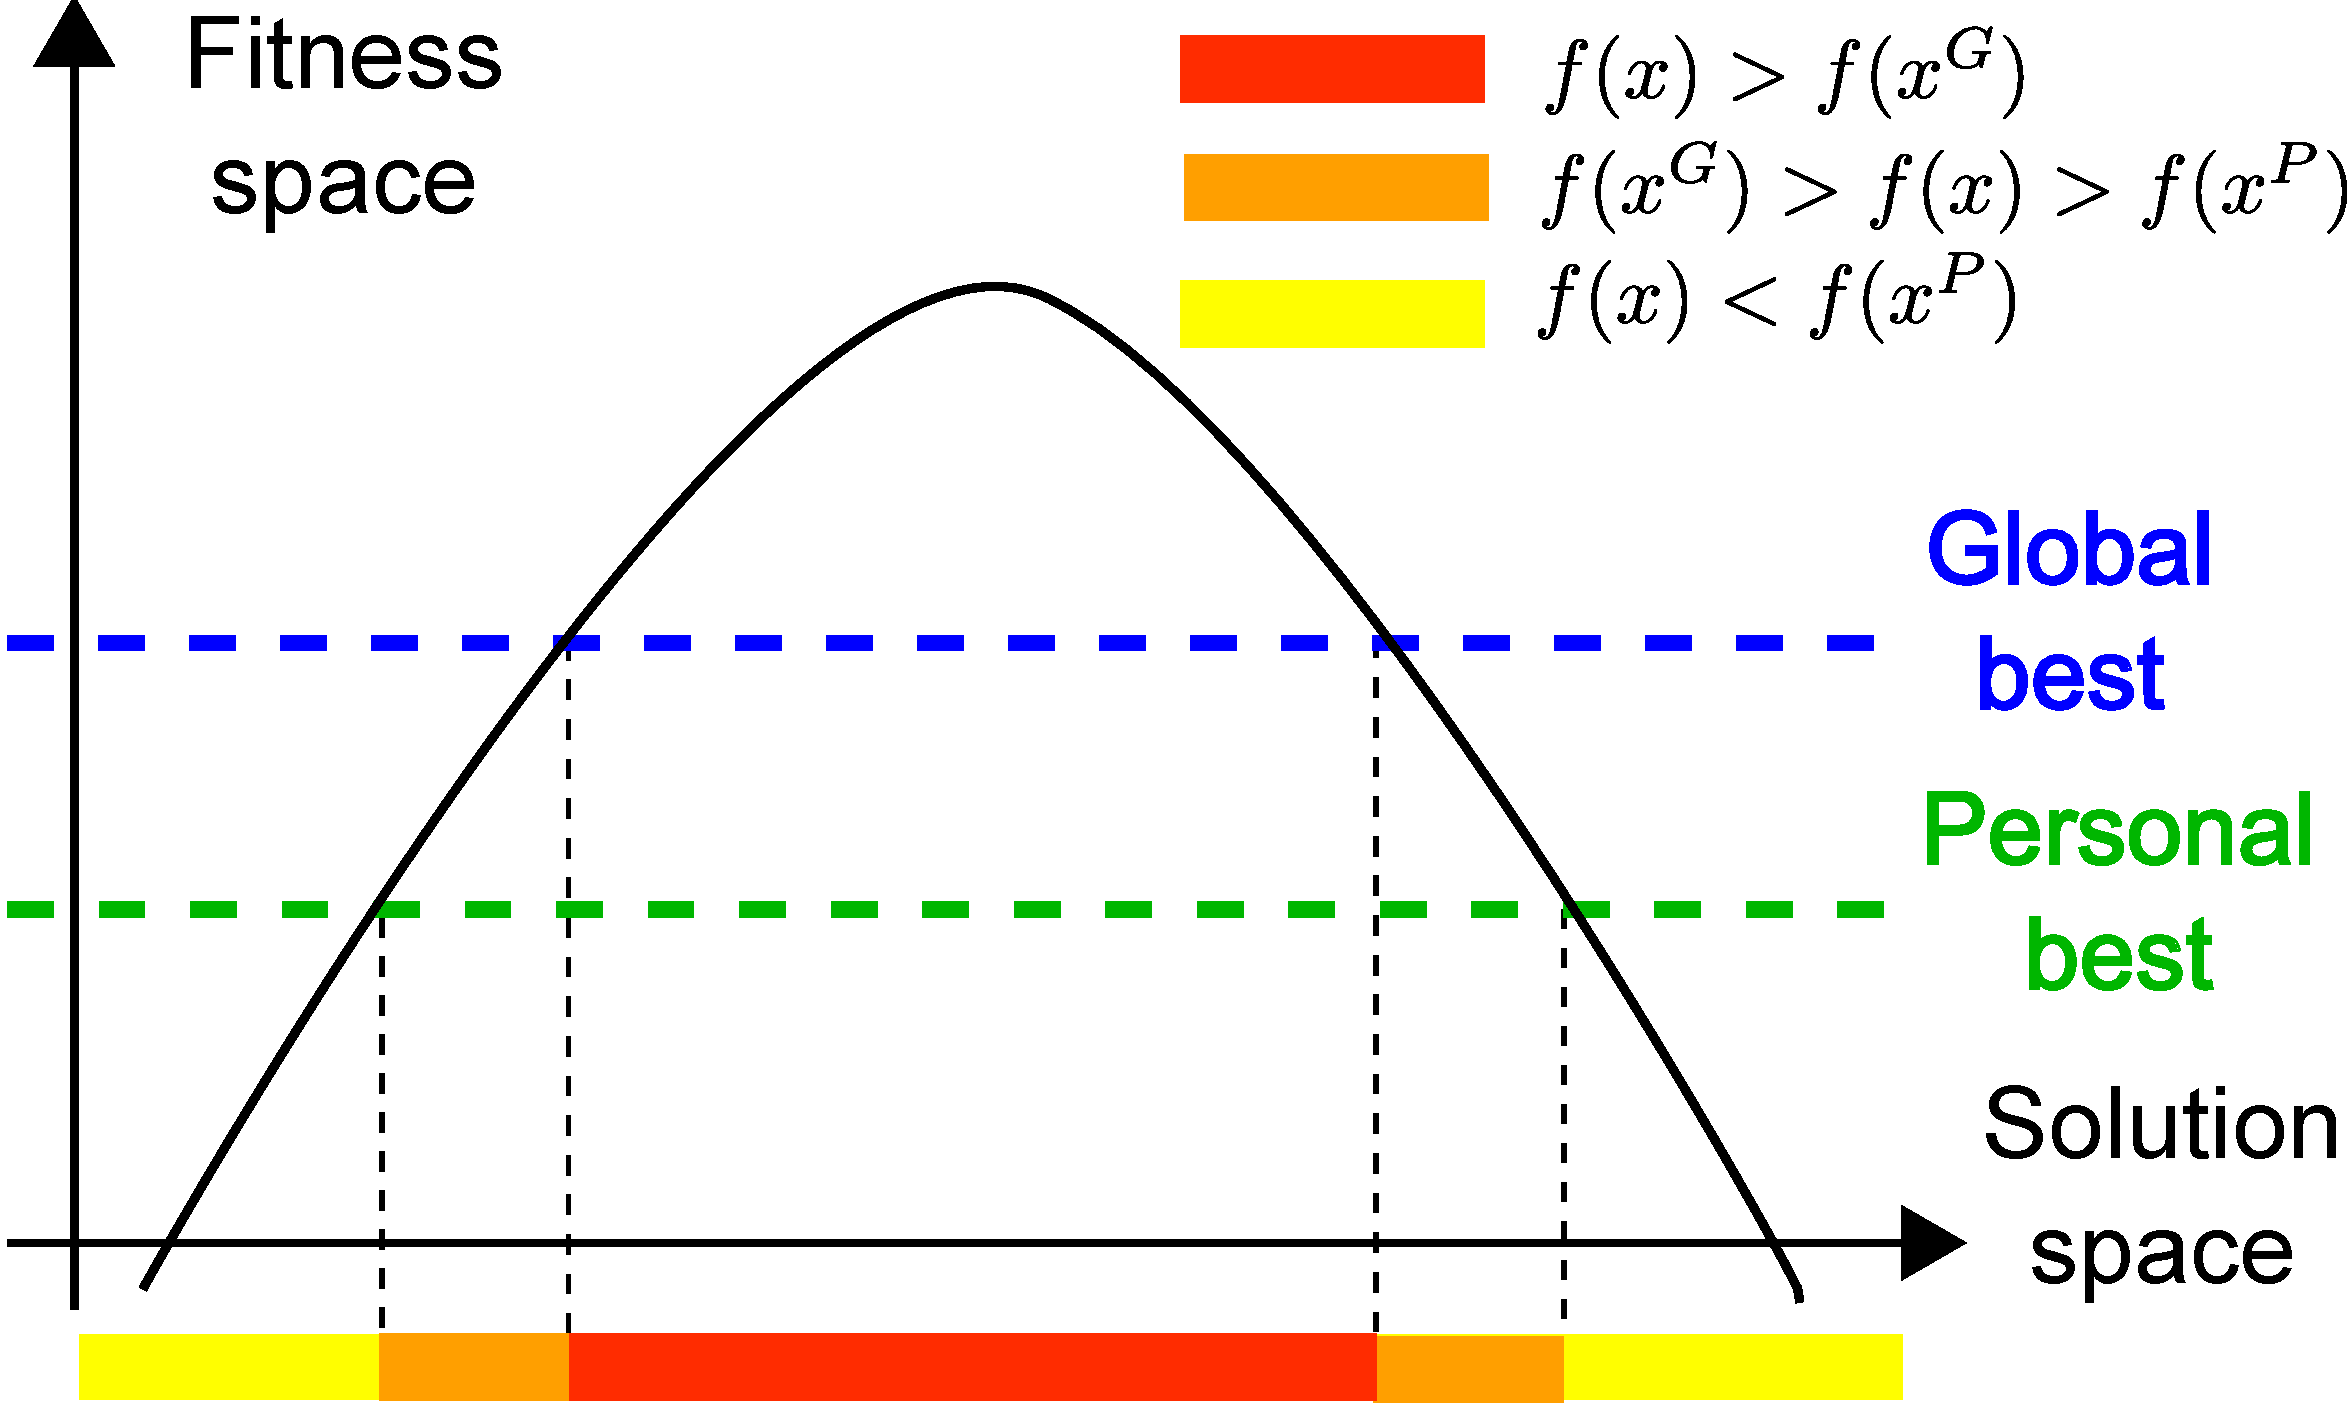
\includegraphics[width=0.7\linewidth]{./fig/categorize_regions}
\caption{How global best and personal best divide the solution space.}
\label{fig:categorize_regions}
\end{figure}

The result of the movement of a particle is determined by which region of the solution space it moves in.
The states of the particle can be defined as
\begin{itemize}
\item \textbf{A} [$ f(x) \leq f(x^{P}) \leq f(x^{G}) $]
\item \textbf{B} [$ f(x) = f(x^{P}) \leq f(x^{G}) $] 
\item \textbf{C} [$ f(x) = f(x^{P}) \leq f(x^{G}) \land v > 0 $]
\item \textbf{D} [$ f(x) = f(x^{P}) \leq f(x^{G}) \land v = 0 $]
\item \textbf{E} [$ f(x) > f(x^{P}) = f(x^{G}) $]
\end{itemize}


\begin{figure}[tbph]
\centering
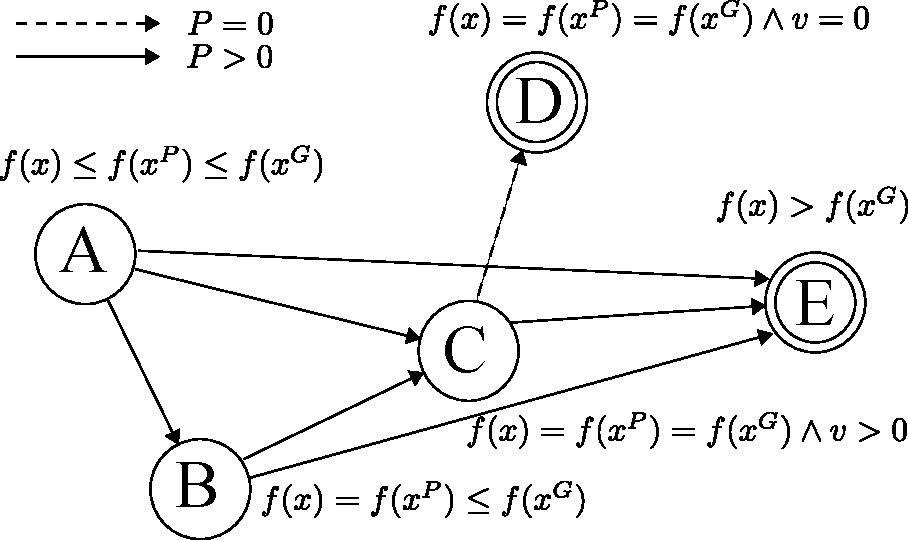
\includegraphics[width=0.7\linewidth]{./fig/fsm}
\caption{}
\label{fig:fsm}
\end{figure}

\end{proof}
\end{mythm}

\subsubsection{Simulation on unimodal case}

\begin{figure}[ht]
\centering
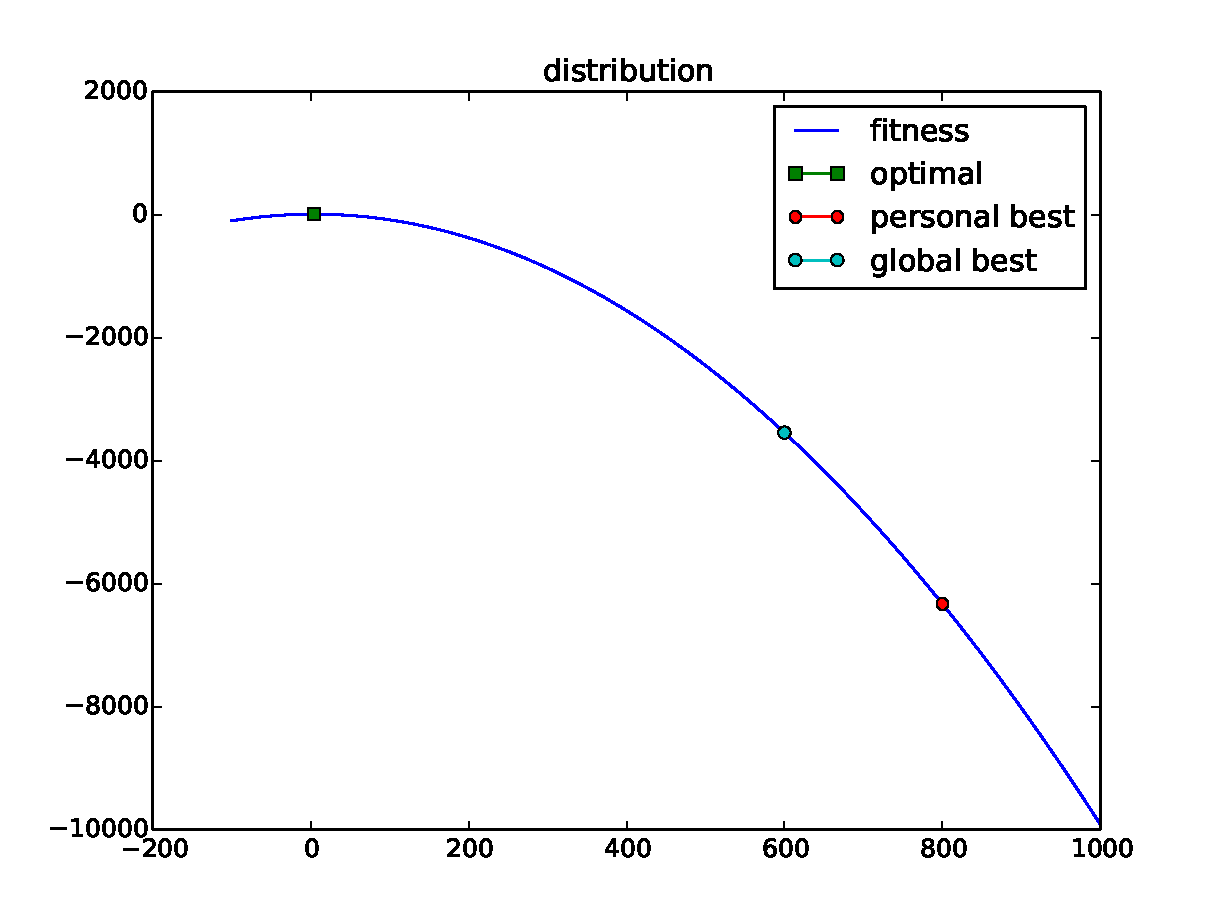
\includegraphics[width=.7\linewidth]{./simfig/case1/distribution1}
\label{fig:case1-1:distribution} 
\end{figure}

\begin{figure}[ht]
\centering
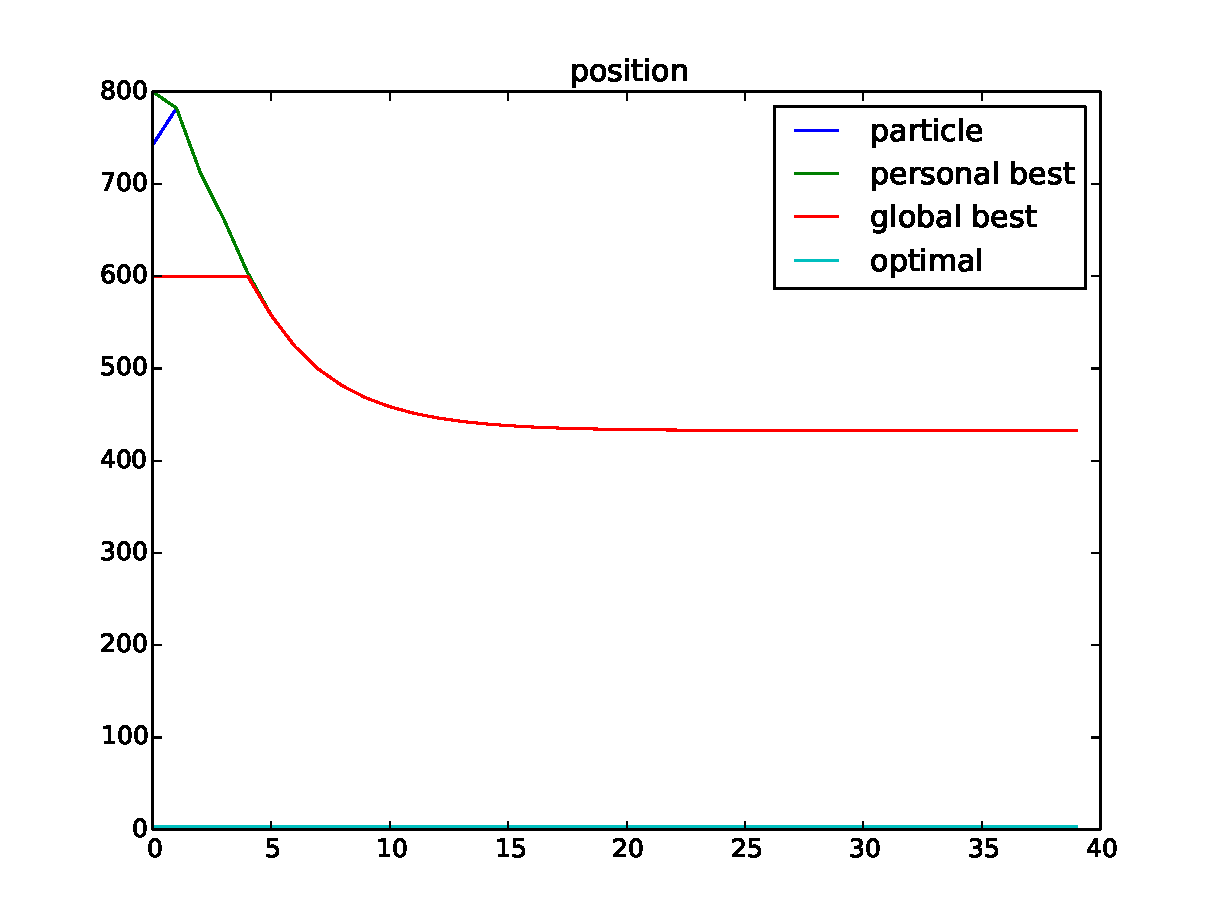
\includegraphics[width=.7\linewidth]{./simfig/case1/position1-1} 
\label{fig:case1-1:position}
\caption{$ \chi = 0.72984 , \phi^{P} = 2.05 , \phi^{G} = 2.05 $ }
\end{figure}

\begin{figure}[ht]
\centering
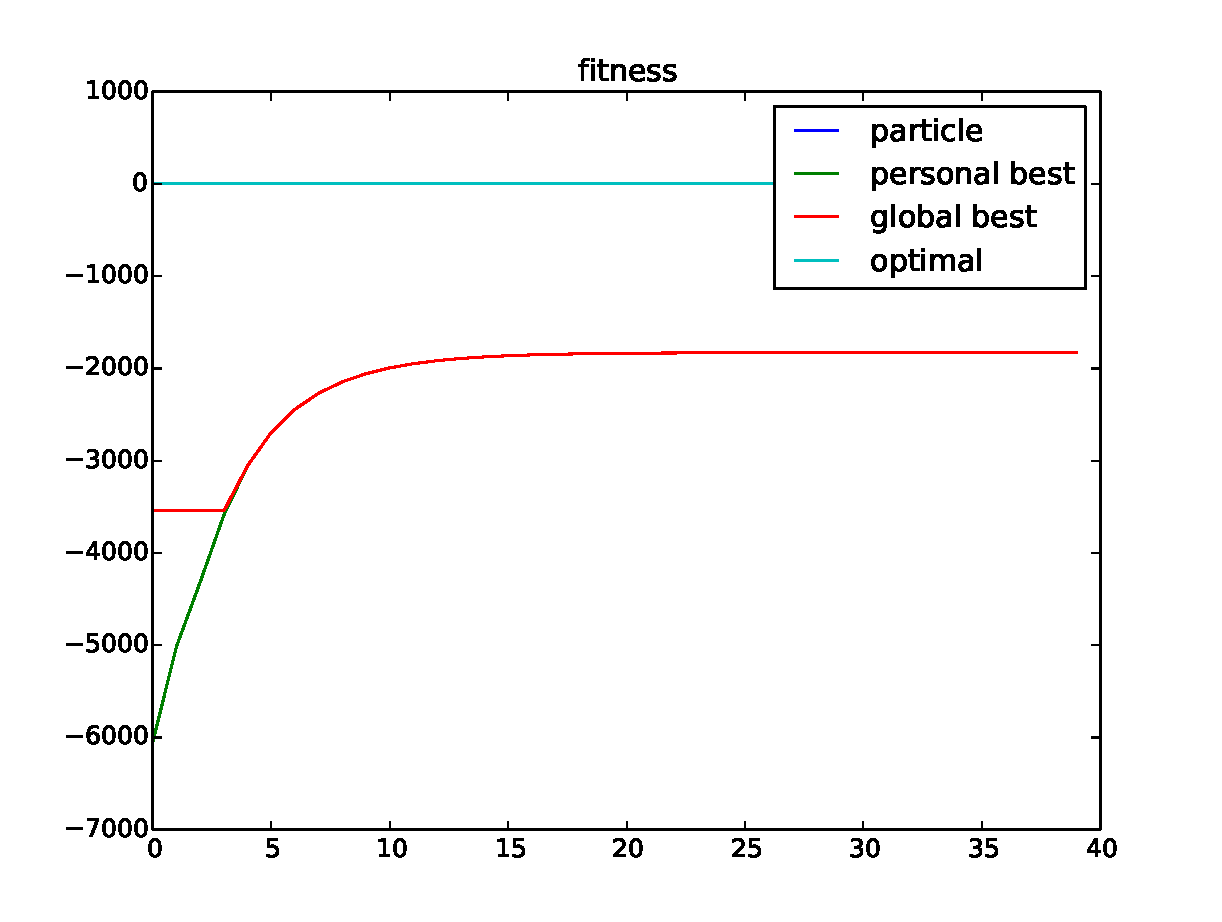
\includegraphics[width=.7\linewidth]{./simfig/case1/fitness1-1} 
\label{fig:case1-1:fitness}
\caption{$ \chi = 0.72984 , \phi^{P} = 2.05 , \phi^{G} = 2.05 $ }
\end{figure}

\begin{figure}[ht]
\centering
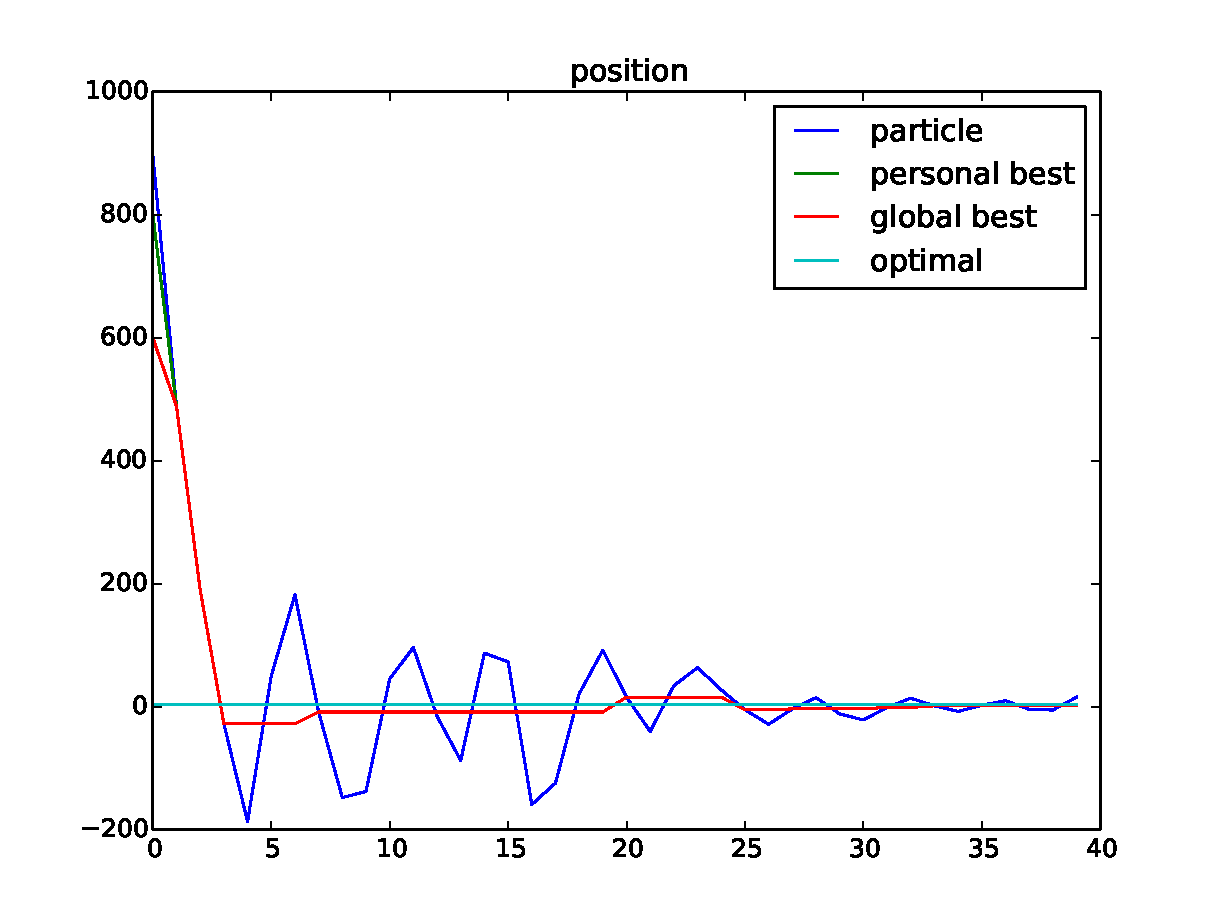
\includegraphics[width=.7\linewidth]{./simfig/case1/position1-2} 
\label{fig:case1-2:position}
\caption{$ \chi = 0.72984 , \phi^{P} = 2.05 , \phi^{G} = 2.05 $ }
\end{figure}
  
\begin{figure}[ht]
\centering
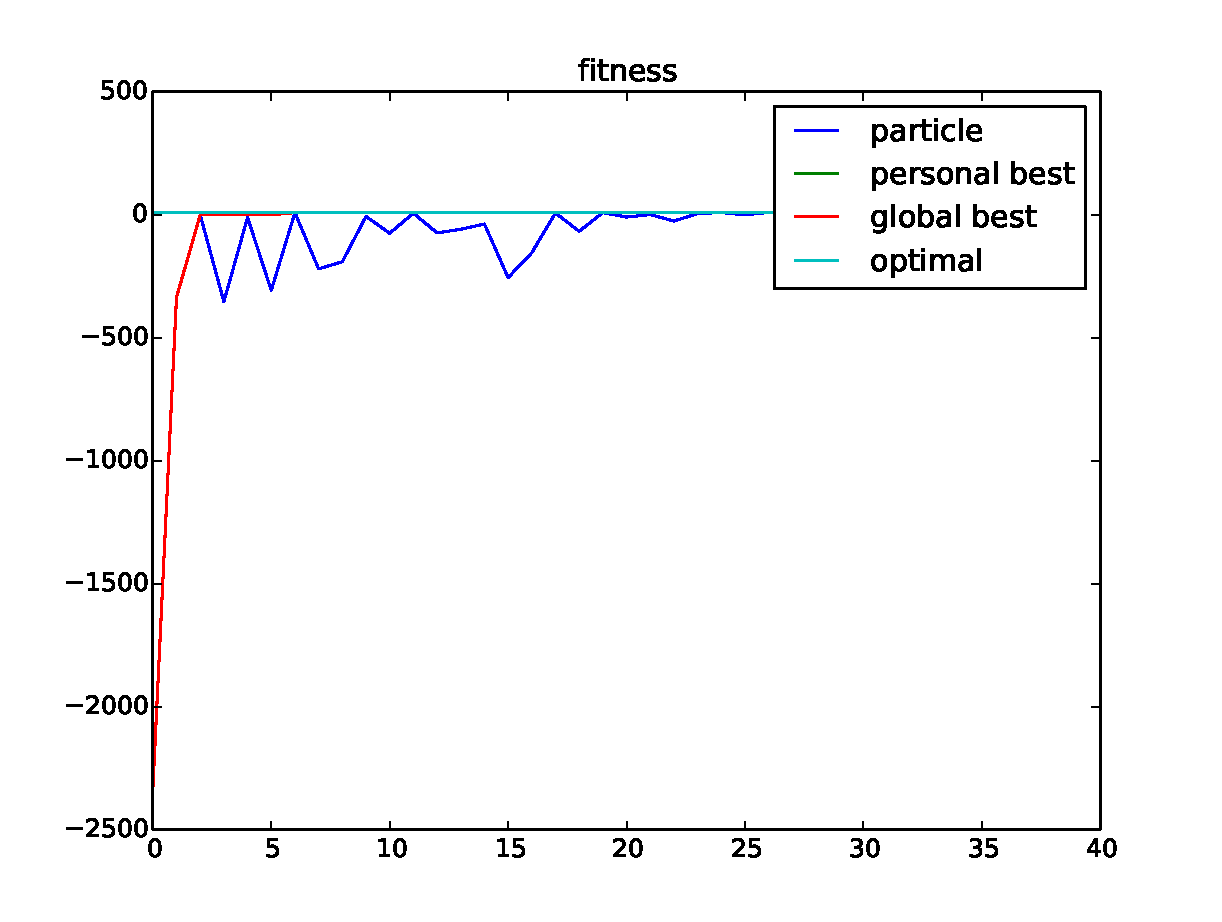
\includegraphics[width=.7\linewidth]{./simfig/case1/fitness1-2} 
\label{fig:case1-2:fitness} 
\caption{$ \chi = 0.72984 , \phi^{P} = 2.05 , \phi^{G} = 2.05 $ }
\end{figure}

\subsubsection{Exploitation}

The convergence property in a unimodal case shows the potential exploitation from the single particle.
As a search heuristic, $ x^{G} $ attracts the particle moving toward itself.


\subsection{Multi-model fitness distribution}

When there is more than one hill in the range that the particle moves, it is not easy to figure out a pattern of the behaviors that the particles share.

[TODO: Give an example that the particle will wander between the personal best and the global best]

As we are interested with the probability that the particle gets into a position that is better than the current global best, we hope the distance from this position to the optimal is closer than that from the global best to the optimal.

In order to measure how likely the particle can moves to a position that $ f(x) > f(x^{G}) $, we can measure the probability of that $ \lVert x(k) - x^{*} \rVert < \lVert x^{G} - x^{*} \rVert $ indirectly.

\begin{mylem}
\label{lem:nonsingleHill:particle:prob}
\begin{equation}
\begin{aligned}
& P( \lVert x(k) - x^{*} \rVert < \lVert x^{G} - x^{*} \rVert ) \\
& > 1 - \frac{ \delta ( \max ( \lVert x^{G} - x^{*} \rVert , \lVert x^{P}(k) - x^{*}  \rVert ) ) }{ \lVert x^{G} - x^{*} \rVert },
\end{aligned}
\end{equation}
in which $ \delta () $ is a boundary function.
\begin{proof}
By Markov's inequality, we have
\begin{equation}
P( \lVert x(k) - x^{*} \rVert \geq \lVert x^{G} - x^{*} \rVert ) \leq \frac{ E( \lVert x(k) - x^{*} \rVert ) }{ \lVert x^{G} - x^{*} \rVert }.
\end{equation} 
By the boundary, we have
\begin{equation}
E( \lVert x(k) - x^{*} \rVert ) \leq \delta ( \max ( \lVert x^{G} - x^{*} \rVert , \lVert x^{P}(k) - x^{*}  \rVert ) ),
\end{equation}
in which $ \delta () $ is the boundary function.
\begin{equation}
\begin{aligned}
& P( \lVert x(k) - x^{*} \rVert < \lVert x^{G} - x^{*} \rVert ) \\
= & 1 - P( \lVert x(k) - x^{*} \rVert \geq \lVert x^{G} - x^{*} \rVert ) \\
> & 1 - \frac{ E( \lVert x(k) - x^{*} \rVert ) }{ \lVert x^{G} - x^{*} \rVert } \\
> & 1 - \frac{ \delta ( \max ( \lVert x^{G} - x^{*} \rVert , \lVert x^{P}(k) - x^{*}  \rVert ) ) }{ \lVert x^{G} - x^{*} \rVert }.
\end{aligned}
\end{equation}
\end{proof}
\end{mylem}

\subsubsection{Simulation on multi-modal cases}

\begin{figure}[ht]
\centering
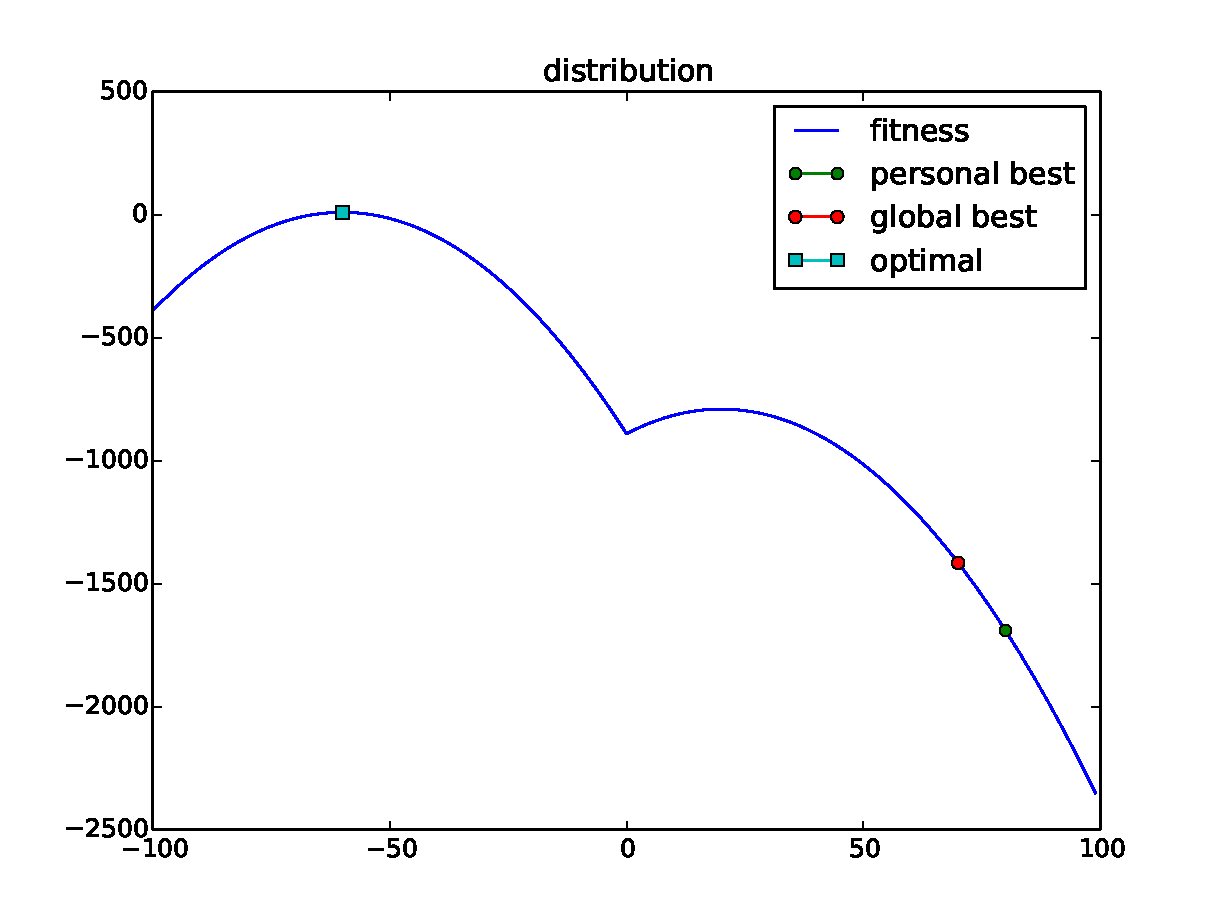
\includegraphics[width=.7\linewidth]{./simfig/case2/distribution2}
\label{fig:case2-1:distribution} 
\end{figure}

\begin{figure}[ht]
\centering
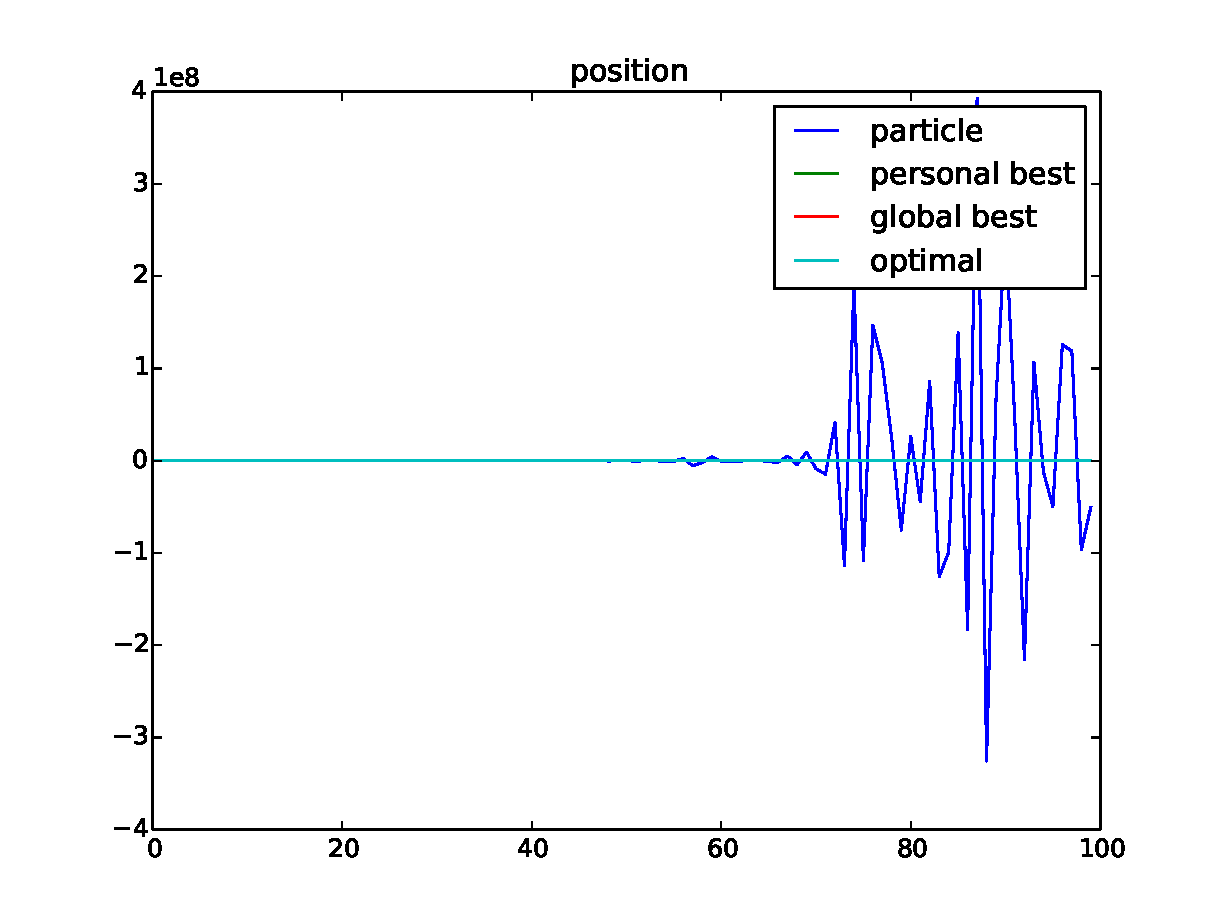
\includegraphics[width=.7\linewidth]{./simfig/case2/position2-1} 
\label{fig:case2-1:position}
\caption{$ \chi = 0.72984 , \phi^{P} = 2.05 , \phi^{G} = 2.05 $ }
\end{figure}

\begin{figure}[ht]
\centering
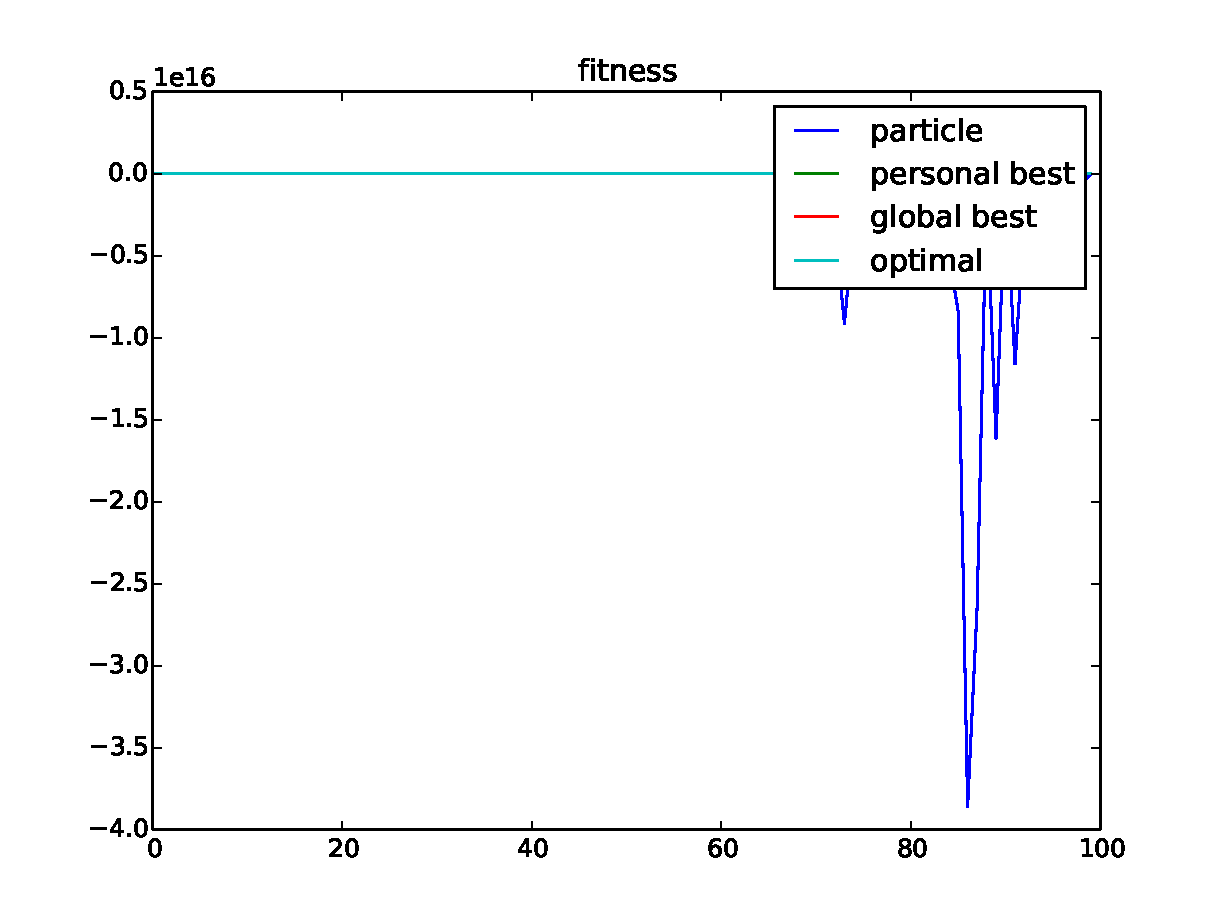
\includegraphics[width=.7\linewidth]{./simfig/case2/fitness2-1} 
\label{fig:case2-1:fitness}
\caption{$ \chi = 0.72984 , \phi^{P} = 2.05 , \phi^{G} = 2.05 $ }
\end{figure}

\begin{figure}[ht]
\centering
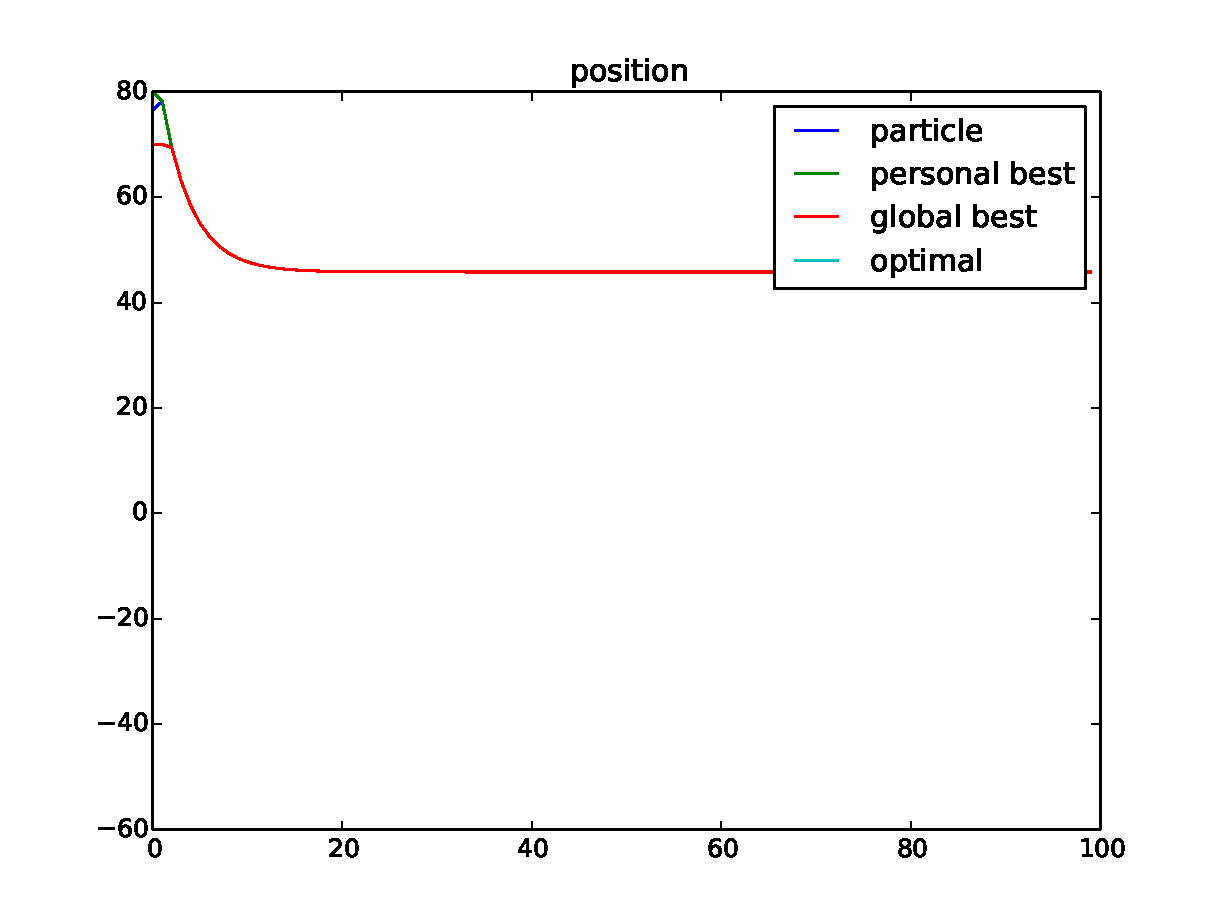
\includegraphics[width=.7\linewidth]{./simfig/case2/position2-2} 
\label{fig:case2-2:position}
\caption{$ \chi = 0.72984 , \phi^{P} = 2.05 , \phi^{G} = 2.05 $ }
\end{figure}
  
\begin{figure}[ht]
\centering
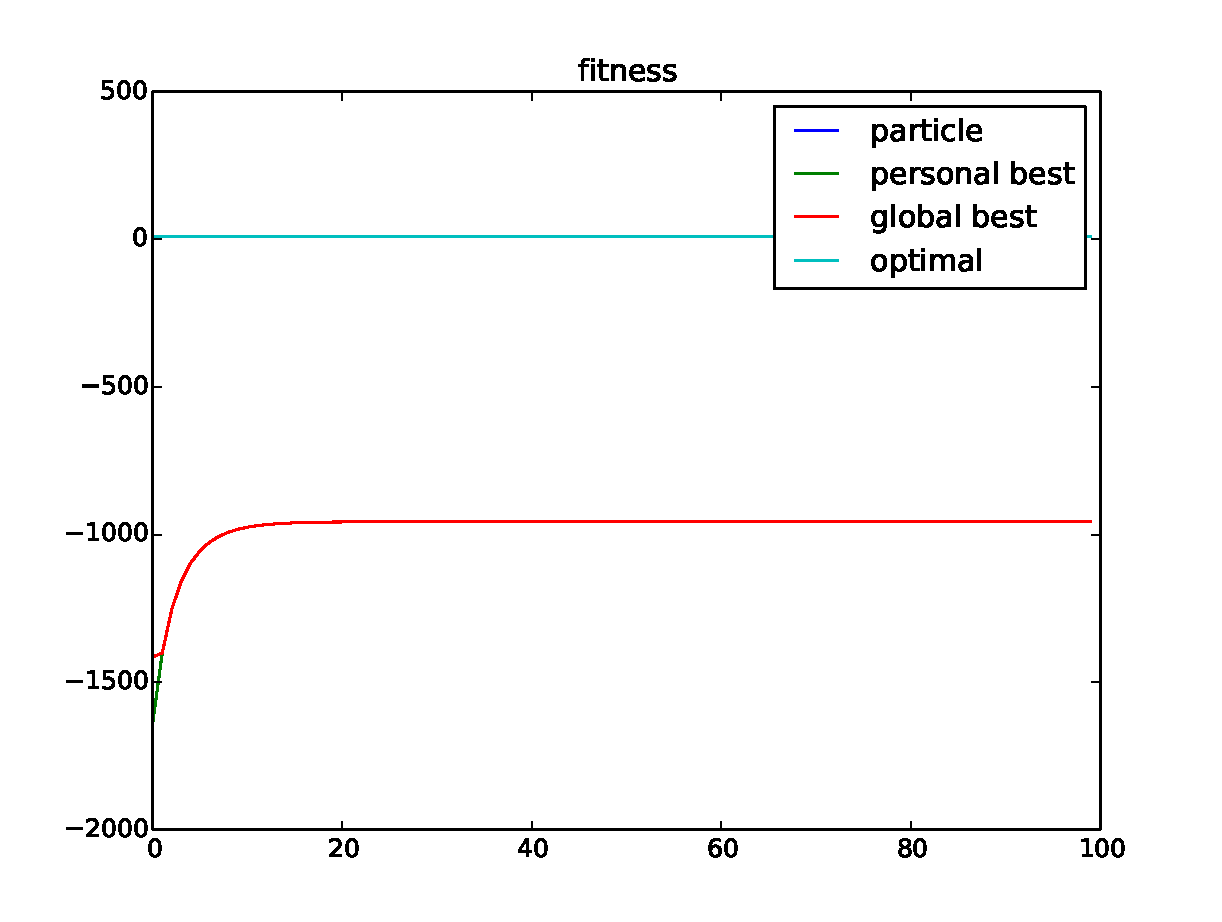
\includegraphics[width=.7\linewidth]{./simfig/case2/fitness2-2} 
\label{fig:case2-2:fitness} 
\caption{$ \chi = 0.72984 , \phi^{P} = 2.05 , \phi^{G} = 2.05 $ }
\end{figure}

\subsubsection{Exploration}


\section{Swarm analysis}
\label{sec:swarm}

%\subsection{Consensus of a swarm}

%\begin{itemize}
%\item Combinations of ISS parts are ISS
%\item Swarm as such a combination
%\item Conditions where update is ISS
%\item trivially at stagnation. But also when on a single hill
%\end{itemize}

%\begin{itemize}
%\item Bound on swarm for the single hill case (perhaps as function of the width of the hill?
%Or width of the hill as a percentage of the feasible region?)
%\item test on 2-d case to show that the bound can prevent a particle from reaching another hill.
%This is one form of the swarm failing to converge the global optimal.
%\item Can we look at parameters for the whole swarm?
%\end{itemize}

\subsection{When the fitness distribution is a single hill}

\begin{mythm}
In one hill case, if there are more than two particles, $ x^{G} \rightarrow x^{*} $.
\begin{proof}
There are two cases, $ x^{G} = x^{*} $ and $ x^{G} \not = x^{*} $
If the global best is $ x^{*} $, the particles will gradually converge to $ x^{*} $ by Lemma \ref{lem:singleHill:particle:nonstop}.
If the global best is not $ x^{*} $, the particles will take turns to find new global best by Theorem \ref{thm:singleHill:particle:better} till $ x^{*} = x^{G} $.
Then it becomes the case $ x^{G} = x^{*} $.
\end{proof}
\end{mythm}

\subsubsection{Simulation}

\subsection{More than single hill case}

\begin{mythm}
The probability that the swarm finds a better global best depends on the probabilities that the particles find better global best, which is
\begin{equation}
P = 1 - \prod_{i=1}^{N} ( 1 - P_{i} ),
\end{equation}
$ P_{i} $ is the probability of particle $ i $ finds a better global best.
\begin{proof}
The search process is a competition among the particles in the swarm.
If the swarm does not find a better global best, it means that none of the particle finds a better global best.
For particle $ i $, the probability that a new global best cannot be found is $ 1 - P_{i} $.
Because the global best is constant, the movements of the particles are independent in the search process.
Thus, the probability that no particle finds a new global best becomes
$ \prod_{i=1}^{N} ( 1 - P_{i} ) $.
Then we can know that the probability that a new global best can be found by the swarm.
\end{proof}
\end{mythm}

\subsubsection{Simulation}

\subsection{Value of a swarm}

%Being on one hill is the unlikely case bound in the multi hill case.
%Might not seem useful but is the essence of what makes a swarm a swarm.
%Bounds the swarm to a region around p-bests where g-best has been unable to pull other particles to its hill.
%For a function with narrow hills, g-bests on a narrow hills is less likely to capture another particle, thus the swarm searches more, for functions with broad hills, p-gest are more likely to be pulled to g-bests hill and search there.
%Thus swarm diversity is the mechanism that allows the swarm to not converge when searching is likely needed but focus and converge when the fitness landscape appear to favor exploitation.
%This does not happen at stagnation and does not happen without multiple members. <need to say this in a more mathematical way>>

%example ?? function for exploration case
%example sphere function for the exploitation case
%try to use bound as a function of hill width metric

%Rastrigin as a counter example? Does it get stuck or just sample for ever? It certainly runs longer.

\subsubsection{Competition}



\subsubsection{Diversity}


\subsection{Diversity injection}

%Work with the Rastrigin function has lead others to experiment with diversity injection to prevent pre-mature convergence (or prevent convergence at all)
%I am not sure, do we want it to converge? ever?
%On what basis would I propose a new algorithm?
%Show that it would converge based on ISS?

\bibliographystyle{IEEEtran}
\bibliography{reference}


\end{document}

